\documentclass[12pt]{article}
\usepackage[left=2cm, right=2cm, top=2cm]{geometry}
\usepackage[utf8]{inputenc} 
\usepackage{mdframed} %For framing the title
\usepackage{graphicx} % to include images
\usepackage{amsmath} % For math mode
\usepackage{mathtools} %for bmatrix*
\usepackage{caption} % For captions
\usepackage{subcaption} % To use caption while using mini page
\usepackage{amssymb} % To use math symbols
\usepackage{multirow} %To combine multiple rows in a table
\usepackage[table]{xcolor} %To color rows / columns in table
\usepackage{titling} %To vertically center the title page
\usepackage{hyperref} %for URL
\usepackage{float} %For [H] in includegraphics
\usepackage[section]{placeins} %PRevents floats before a section
\usepackage{textcomp} %For degree symbol


%----------------------------MATLAB TEMPLATE -------------------------------------
\usepackage{listings}
\usepackage{color} %red, green, blue, yellow, cyan, magenta, black, white
\definecolor{mygreen}{RGB}{28,172,0} % color values Red, Green, Blue
\definecolor{mylilas}{RGB}{170,55,241}
%-----------------------------------------------------------------------------------------

\title{ECE 8540 \\ Analysis of Tracking Systems \\ \quad \\
	Assignment 6 \\ Particle Filter}
\author{Vivek Koodli Udupa \\ C12768888}
\date{November 20, 2018 }

%%To make the title page center vertically centered
%\renewcommand\maketitlehooka{\null\mbox{}\vfill}
%\renewcommand\maketitlehookd{\vfill\null}

\begin{document}
\begin{mdframed}
%Displaying Title
%\begin{titlepage}
\maketitle
%\pagenumbering{gobble}% Remove page numbers (and reset to 1)
%\end{titlepage}
\end{mdframed}
\pagenumbering{arabic}% Arabic page numbers (and reset to 1)


%Begin of Report
\section{Introduction}
This report considers the problem of tracking a non-linear model with generalized noise distribution using Particle Filter. In filtering, there are two prominent equations that describe the model that was designed to address a problem. The two equations are observation equation and state transition equation. The observation equation describes the measurements that are obtained through the sensors and the state transition equation describes how the system is expected to change over time. Kalman and Extended Kalman Filters are generally used for such tracking problems. However, Kalman filter is only indented for linear systems. The extended Kalman filter works on nonlinear systems. Both filters assume that the state distribution, dynamic noise and observation noise are all Gaussian. In order to track a more generalized non-linear non-Gaussian distribution Particle Filter is preferred which uses a genetic mutation-selection sampling approach, with a set of particles (also called samples) to represent the posterior distribution of some stochastic process given noisy and/or partial observations. The state-space model can be nonlinear and the initial state and noise distributions can take any form required.\\ 
\\ \indent
A distribution is called \lq\lq{intractable}\rq\rq{} if it is not easily modelled by an analytical function, or that even if it can be modelled, the function does not provide an easy mechanism for calculation. In order to deal with such distributions, Monte Carlo approximation is used. Monte Carlo approximation is the practice of using a set of samples to approximate a distribution. Each sample is given a state and a weight. These samples are simply a \lq\lq{guess}\rq\rq{} at the actual state of the object being tracked. Weighing each guess for its accuracy is difficult. To work around this problem importance sampling is used. The idea behind importance sampling is that certain values of the input random variables in a simulation have more impact on the parameter being estimated than others. If these "important" values are emphasized by sampling more frequently, then the estimator variance can be reduced. Thus with enough samples, weighted and positioned appropriately, any distribution can be approximated.  \\ 
\\ \indent
In general tracking problems, the desire is to determine the probability of all transitions over time given all the observations. However, realistically it is better to set up a recursive relationship where the next estimate is based on the previous estimate and the latest measurement. The recursive Bayesian estimation helps us to set up such a relationship. \\ 
\\ \indent
This report is focused on tracking an object moving back and forth along a string. Two magnets are placed at fixed positions near the string. The object senses the magnetic field strength. Given the magnetic field measurement, the position of the object is to be tracked. In other words, what is the probability of position of the object given a field strength? This question is addressed in this report using a Particle Filter designed based on the concepts of Bayesian estimation, Monte Carlo approximation and sequential importance sampling.  

\section{Methods}
Particle Filter(PF) is a continuous cycle of predict and update. When formulating the problem for the PF following steps are considered:
\begin{enumerate}
	\item Determine the state variables.
	\item Write the state transition equations i.e. How things evolve over time.
	\item Define the dynamic noise(s).  This describes the uncertainties in state transition equation.
	\item Determine the observation variables i.e. Sensor readings.
	\item Write the observation equations (relating the sensor readings to the state variables).
	\item Define the measurement noise(s). These are the uncertainties in observation variables.
	\item Characterize the state transition matrix and observation matrix.
\end{enumerate}

\subsection{Describing the Particle Filter Parameters}
Putting together the concepts of Bayesian estimation, Monte Carlo approximation and sequential importance sampling, particle filter can be described. \\
As with all other filters, the first step is to define the model that will be used in this problem. This model includes the following: 
\begin{enumerate}
\item $X_t$, a set of state variables
\item $a_t$, the set of dynamic noises
\item f(), the state transition equation
\item $y_t$, the set of measurements
\item $n_t$, the set of measurement noises
\item g(), the observation equation
\end{enumerate}

\subsection{Defining the Particle Filter}
The dataset "magnets-data.txt" consists of sensor readings of magnetic field strength experienced by an object hovering over two magnets. The system consists of a 1D position, moving on a line. The system follows a motion pattern where the position `zig-zags' back and forth on a line. The sensor on the system detects a field strength that is the sum of the distances from two fixed-position magnets. The objective is to track the position of this object based on the magnetic field strength readings.\\
\\ 

The problem in hand comprises of two state variables:
\begin{equation}
X_t = \begin{bmatrix}
x_t \\
\dot{x}_t
\end{bmatrix}
\label{eq:States}
\end{equation}
Where $x_t$ is the position of the object and $\dot{x_t}$ represents the velocity of the object.\\  

The state transition equation is as follows:
\begin{equation}
f(x_t,a_t) = \begin{bmatrix*}[l]
x_{t+1} = x_t + \dot{x}_t T \\
\dot{x}_{t+1} = \left\{
\begin{array}{l l}
  2 & \quad \text{if $x_t < -20$} \\
  \dot{x}_t + |a_t| & \quad \text{if $-20 \le x_t < 0$} \\
  \dot{x}_t - |a_t| & \quad \text{if $0 \le x_t \le 20$} \\
  -2 & \quad \text{if $x_t > 20$} \\
\end{array} \right.
\end{bmatrix*}
\label{eq:ST}
\end{equation}
The velocity equation is a piecewise function that adds or subtracts a random amount $a_t$ to the current velocity, depending on the current position. The values $a_t$ are drawn from a zero-mean Gaussian distribution $N(0,\sigma_a^2)$ where $\sigma_a = 0.0625$ . $a_t$ represents the dynamic noise.\\

The observation equation for this model is:
\begin{equation}
g(x_t,n_t) = \begin{bmatrix}
y_t = \frac{1}{\sqrt{2 \pi} \sigma_m}
\mathrm{exp} ( \frac{-(x_t - x_{m1})^2}{2 \sigma_m^2} ) +
\frac{1}{\sqrt{2 \pi} \sigma_m}
\mathrm{exp} ( \frac{-(x_t - x_{m2})^2}{2 \sigma_m^2} ) + n_t
\end{bmatrix}
\label{eq:obs}
\end{equation}
where $n_t$ is a random sample drawn from $N(0,\sigma_n^2)$ representing measurement noise. The value of $\sigma_m = 4.0$ and $\sigma_n = 0.003906$.\\

Since the particle filter is a Monte Carlo approximation, the distribution
$p(x|y)$ is represented using a number of samples.  In the context of
the particle filter, the samples are usually called particles.
They are denoted as:
\begin{equation}
\chi = \lbrace x^{(m)}, w^{(m)} \rbrace ^M_{m=1}
\end{equation} 
where $x^{(m)}$ represents the state of particle $m$ and
$w^{(m)}$ represents the weight of particle $m$.
Here M represents the number of particles to be used. \\

The predict-update cycle for the given problem goes as follows:
\begin{enumerate}
	\item Each particle is propagated through the state transition equation
	\begin{equation}
		\lbrace x_t^{(m)} = f(x_{t-1}^{(m)},a_t^{(m)}) \rbrace ^M_{m=1}
		\label{eq:particleTrans}
	\end{equation}
	The value $a_t^{(m)}$ represents the dynamic noise from time t - 1 to t. This is randomly and independently calculated for individual particle separately. This can be viewed as each particle taking a random guess at the dynamic noise undertaken for the current iteration. \\
	
	\item Using the new measurement vector $y_t$, the weight of each particle is updated. 
	\begin{equation}
	\tilde{w}_t^{(m)} = w_{t-1}^{(m)} \cdot p(y_t | x_t^{(m)})
	\label{eq:weightUpdate}
	\end{equation}
	This weight update equation is based upon selecting the importance distribution as the prior importance function. 			Other choices for the importance distribution lead to different formulations for the weight update equation.\\
	The value $p(y_t | x_t^{(m)})$ is determined by the measurement noise.
	It should be calculated by taking the ideal measurement of the particle, and comparing it against the actual 		     	measurement, in the model of the measurement noise. The ideal measurement of the particle is calculated as follows:
	\begin{equation}
		g(x_t^{(m)},0) = \begin{bmatrix}
		y_t^{(m)} = \frac{1}{\sqrt{2 \pi} \sigma_m}
		\mathrm{exp} ( \frac{-(x_t^{(m)} - x_{m1})^2}{2 \sigma_m^2} ) +
		\frac{1}{\sqrt{2 \pi} \sigma_m}
		\mathrm{exp} ( \frac{-(x_t^{(m)} - x_{m2})^2}{2 \sigma_m^2} )
		\end{bmatrix}
	\end{equation}
	The ideal measurement can then be compared against the actual
	measurement in the model of the measurement noise as follows:
	\begin{equation}
		p(y_t | x_t^{(m)}) = 
		\frac{1}{\sqrt{2 \pi} \sigma_n}
		\mathrm{exp} ( \frac{-(y_t^{(m)} - y_t)^2}{2 \sigma_n^2} )
	\end{equation}
	
	\item Normalize the updated weights:
	\begin{equation}
		w_t^{(m)} = \frac{\tilde{w}_t^{(m)}}{\sum_{m=1}^M \tilde{w}_t^{(m)}}
		\label{eq:weightNormalize}
	\end{equation}
	The normalized weights must sum up to 1.
	
	\item Compute the desired output:
	\begin{equation}
		E[x_t] \approx \sum_{m=1}^M x_t^{(m)} \cdot w_t^{(m)}
		\label{eq:exp}
	\end{equation}
	
	\item Check and re-sample if necessary.\\
	 The co-efficient of variation statistic can be calculated which helps in deciding if re-sampling is necessary. \\
	\begin{equation}
		CV = \frac{1}{M} \sum_{m=1}^{M}\lbrace M \cdot w^{(m)} - 1 \rbrace ^ 2
		\label{eq:CV}
	\end{equation} 
	
	The effective sample size can be calculated as 
	\begin{equation}
		ESS = \frac{M}{1 + CV}
		\label{eq:ESS}
	\end{equation}
	The effective sample size describes how many particles have appreciable weight. In order to check if re-sampling is necessary, the effective sample size can be tested against the number of particles. \\
	In the context of this report, the threshold is set to 50\% of the total particles used i.e M = 1000.
	\begin{verbatim}
  		if (ESS < 0.5 M)
    	resample
	\end{verbatim}	
	
	The most common re-sampling method is called the select with replacement. The concept here is to eliminate particles with negligible weights are replace them with particles that have large weights. The pseudo code for re-sampling is given below:
\begin{verbatim}
  Assume particle states in P[1...M], weights in W[1...M].

  Q=cumsum(W);          calculate the running totals  
  t=rand(M+1);          t is an array of M+1 uniform random numbers 0 to 1
  T=sort(t);            sort them smallest to largest
  T[M+1]=1.0;           boundary condition for cumulative hist
  i=j=1;                arrays start at 1
  while (i<=M)
    if (T[i] < Q[j])
      Index[i]=j;
      i=i+1;
    else
      j=j+1;
    end if
  end while

  loop (i=1; i<=M; i=i+1)
    NewP[i]=P[index[i]];
    NewW[i]=1/M;
  end loop
\end{verbatim}
	This algorithm computes a list of indices of particles. The list may include 1 or more copies of the same index (particle). It may also skip over 1 or more indices (particles). After computing the list, it creates a new list of particles of equal weights. \\
	
	\item Final step is to increment t, i.e t = t + 1 and then iterate.
\end{enumerate}
All of the above implementation has been done in MATLAB. Refer Appendix for the implementation Code. 
\section{Result}
This section consists of plots resulting from the implementation shown above. \\

\begin{figure}[b]
\centering
	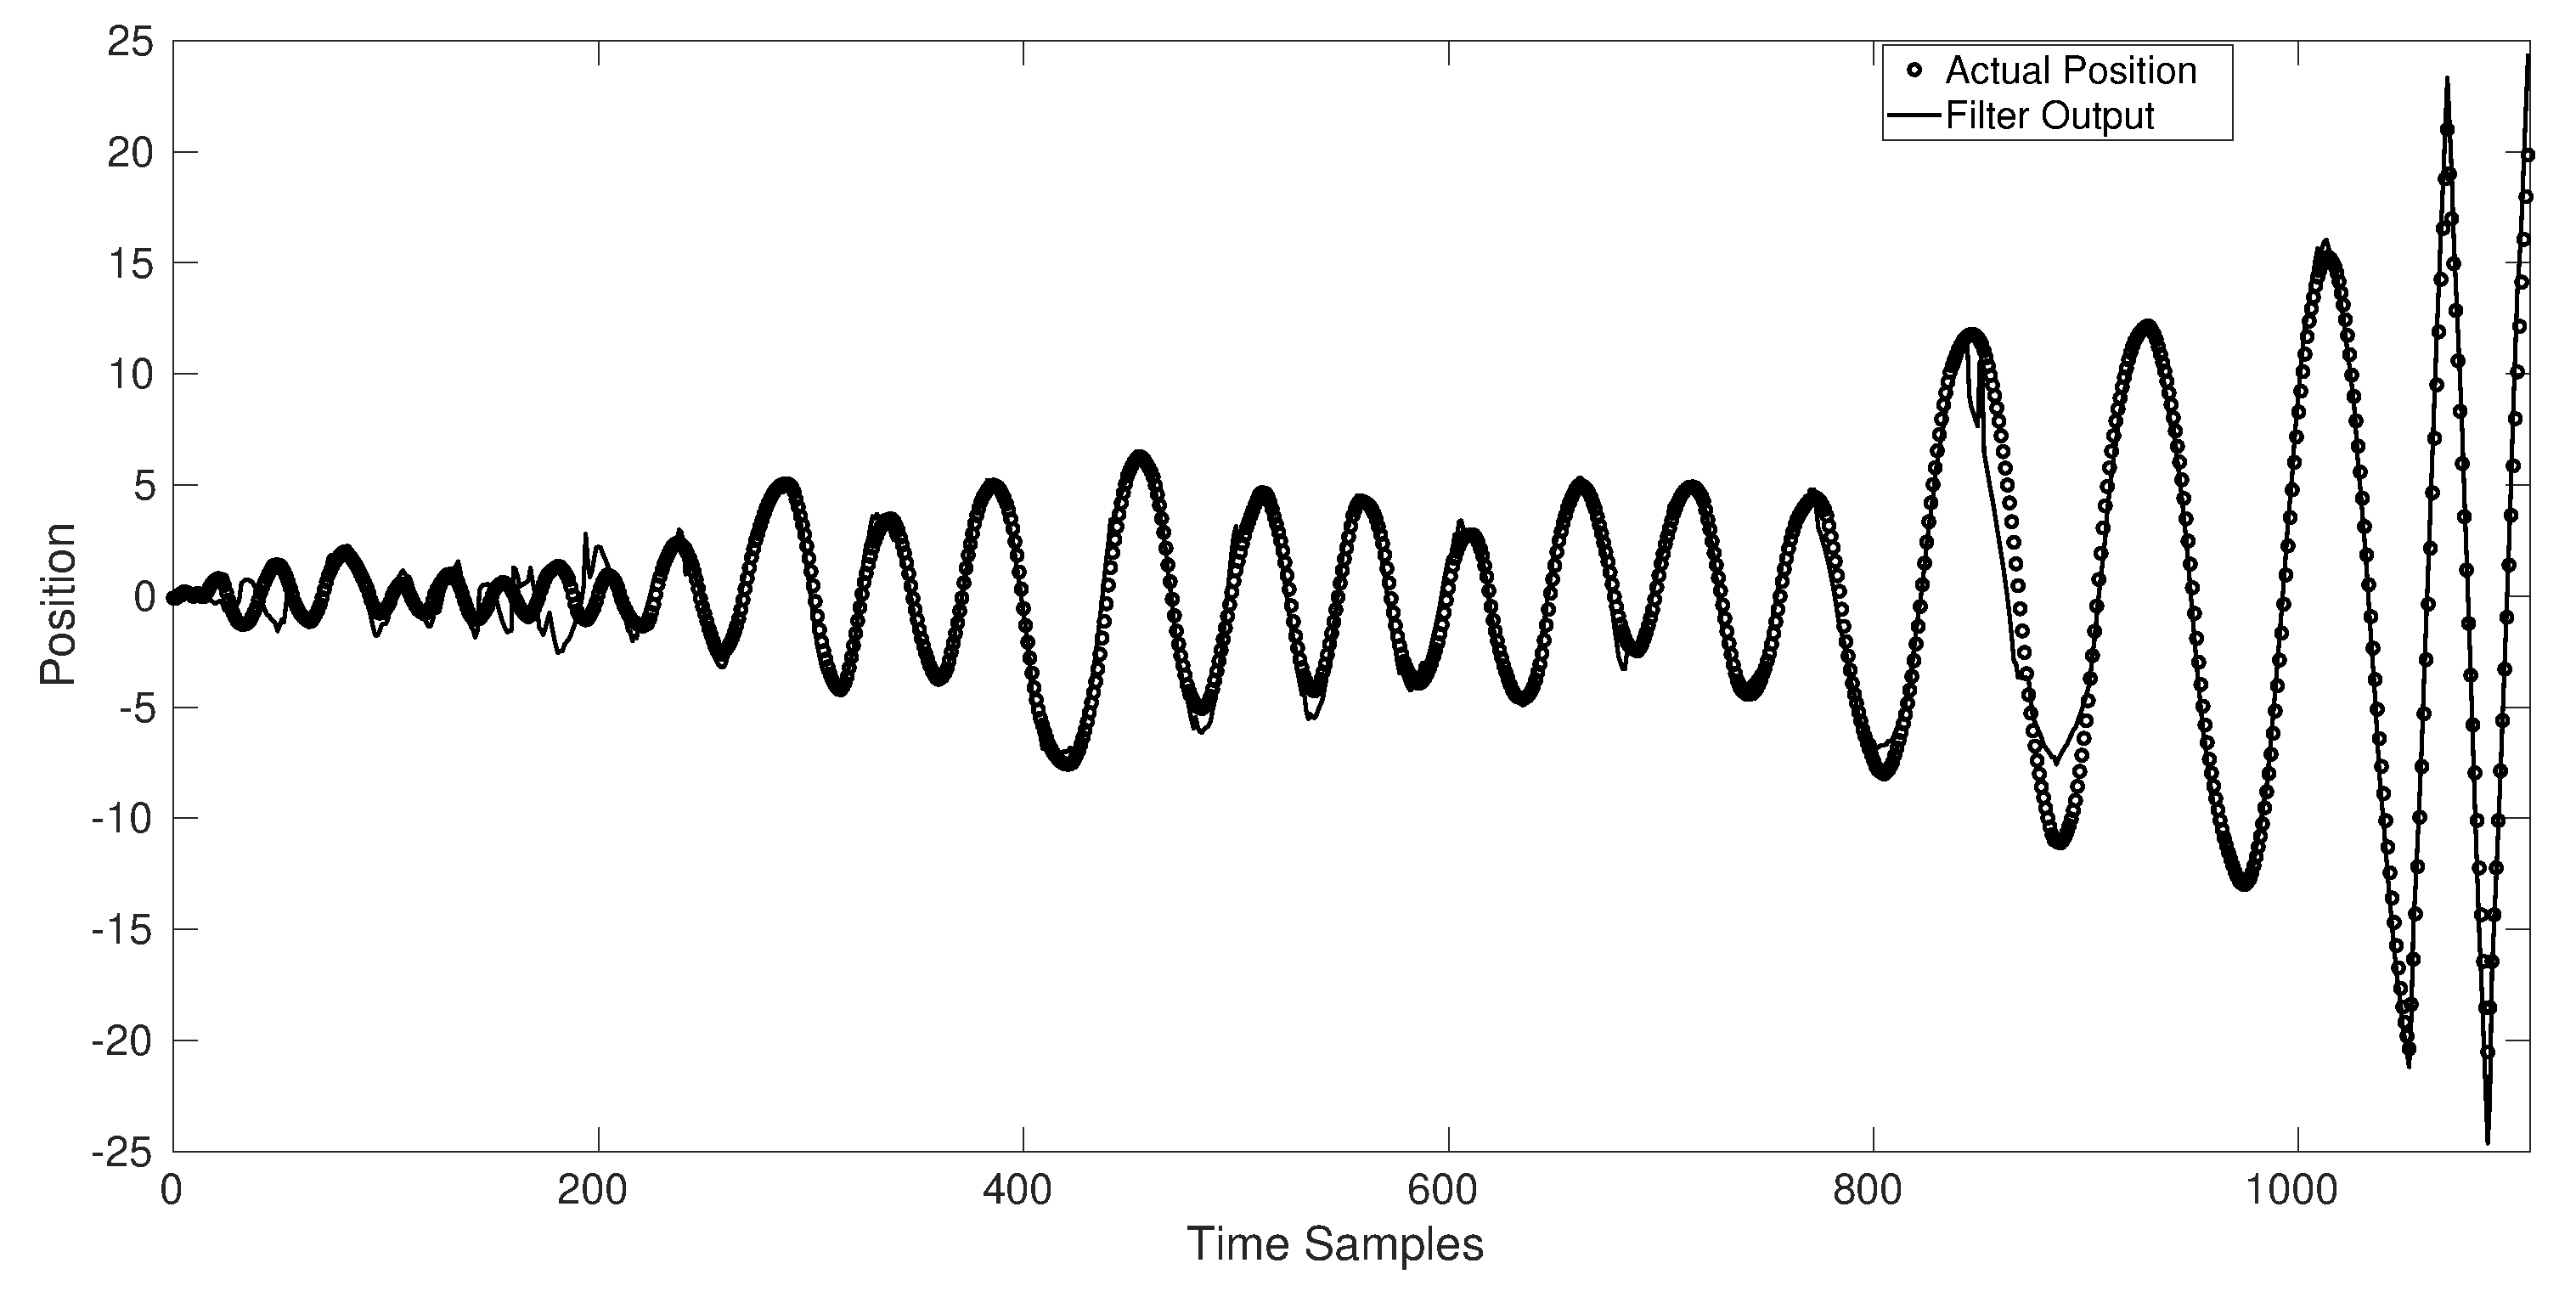
\includegraphics[scale = 0.3]{./Figures/inphase.eps}
	\caption{In-phase tracking}
	\label{fig:inphase}
\end{figure}

\begin{figure}[t]
\centering
	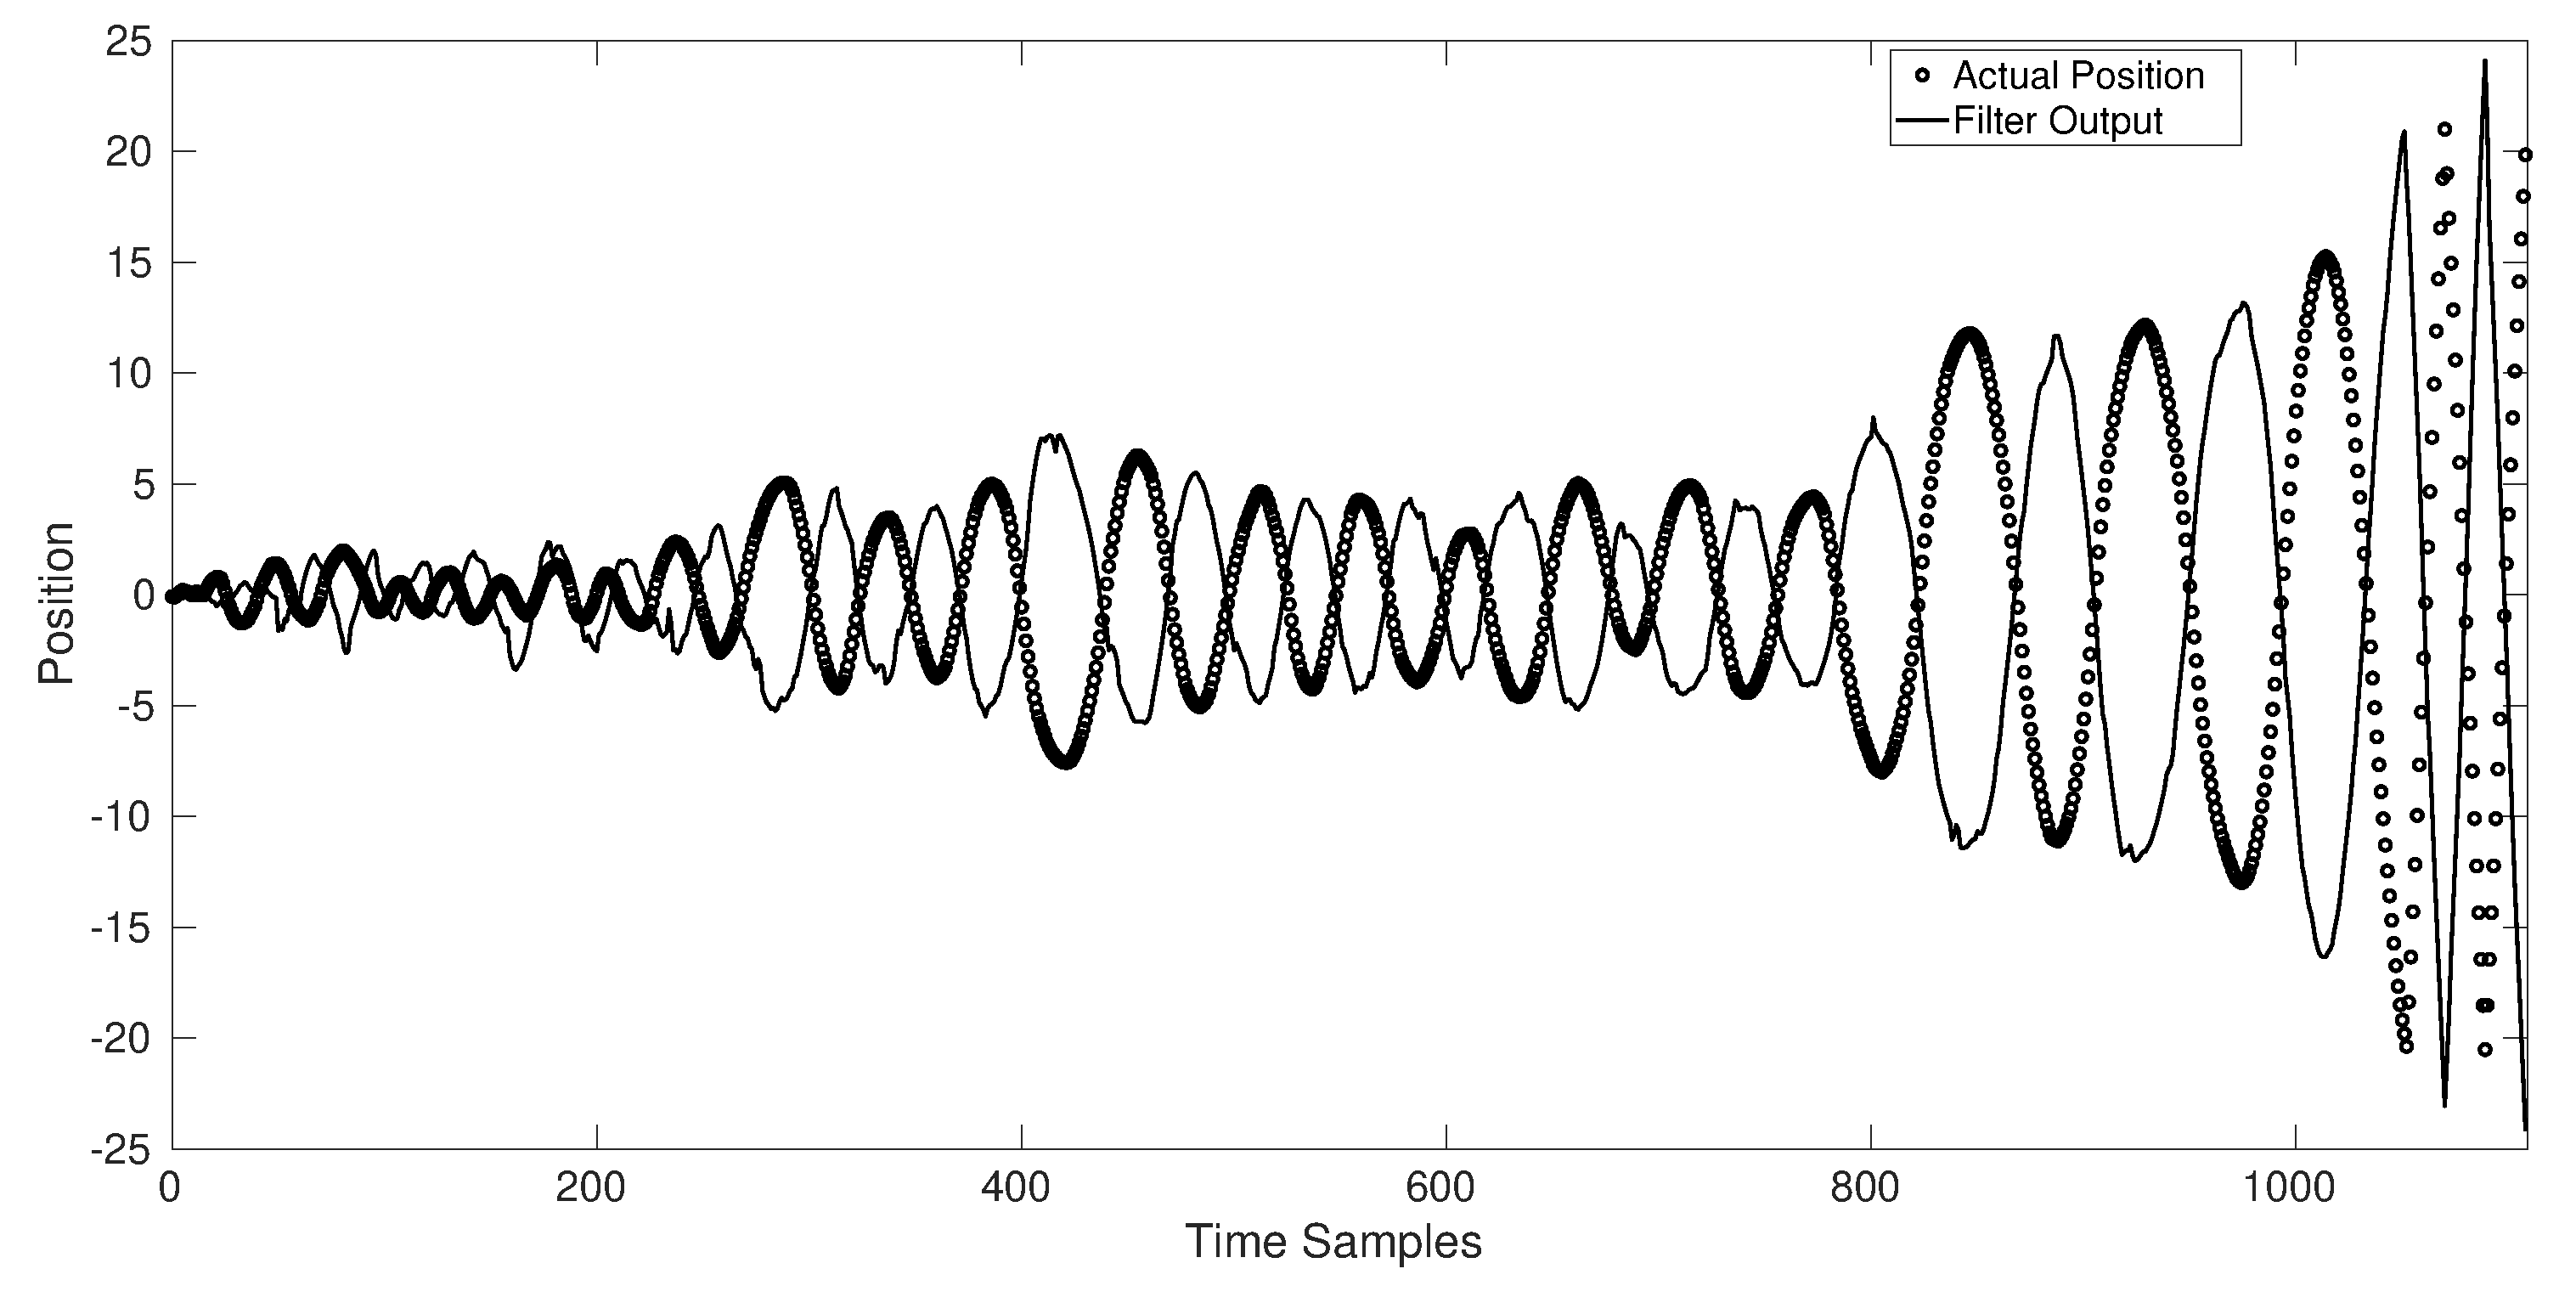
\includegraphics[scale = 0.3]{./Figures/outphase.eps}
	\caption{Out-of-phase tracking}
	\label{fig:outphase}
\end{figure}

Figure \ref{fig:inphase} and Figure \ref{fig:outphase} shows the plot of actual position of the object vs the filter's prediction of the position of the particle. The filter takes some time to lock on to the object. This can be observed in the initial iterations where the filter is having trouble predicting the position of the object. After around 300 iterations, the filter starts to track the object more accurately.\\

In Figure \ref{fig:inphase} The actual position of the object and the filter's prediction of the object's true position are in-phase. This means that the actual position of the object is where the filter is predicting it to be.\\

Figure \ref{fig:outphase} represents out-of-phase tracking where the filter's prediction is off by 180\textdegree. Here the actual position of the object is opposite to where the filter is predicting it to be. \\

Figure \ref{fig:DGweights1} and Figure \ref{fig:DGweights2} represent the normalized weight distribution over the span of one re-sampling cycle. \\
These plots are taken from iteration 120 through iteration 132 where 120 and 132 are the re-sampled iterations. The plot consists of normalized weights that add up to 1. After re-sampling the weights are re-initialized to $\frac{1}{M}$(M = 1000 in this case). ESS represents the number of particles that are still contributing to the approximation of the distribution. It can be observed that this number drops through each iteration and the re-sampling is performed when ESS drops below 50\% of the total number of particles, M. In this case re-sampling is done whenever ESS drops below 500. It can also be observed that the weight distribution takes the form of a double Gaussian.  



\begin{figure}[ht!]
\centering
	\begin{minipage}{0.5\textwidth}
		\centering
		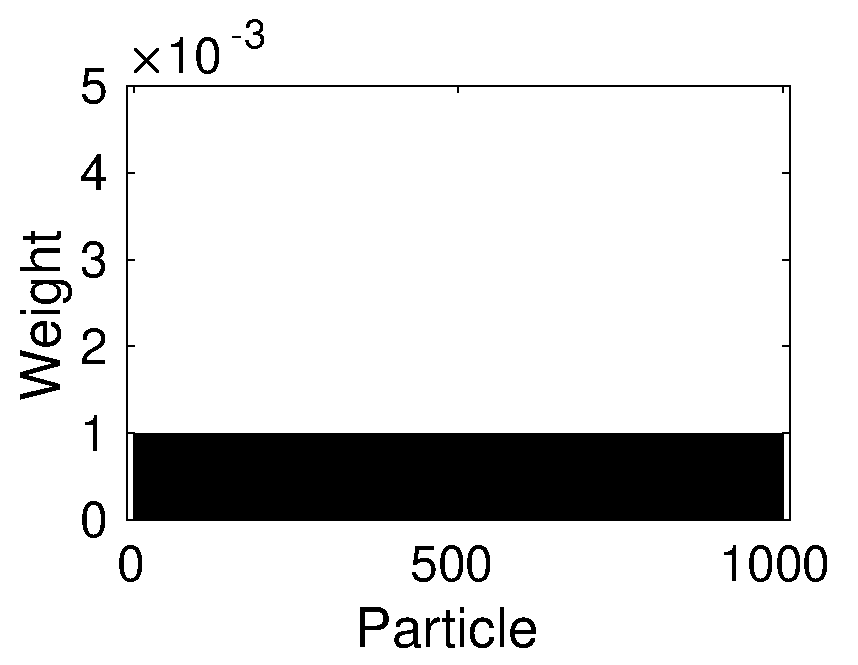
\includegraphics[scale = 0.5]{./Figures/120resampled.eps}
		\caption*{Iterations = 120 ESS = 381.7177}
	\end{minipage}% 
	\begin{minipage}{0.5\textwidth}
		\centering
		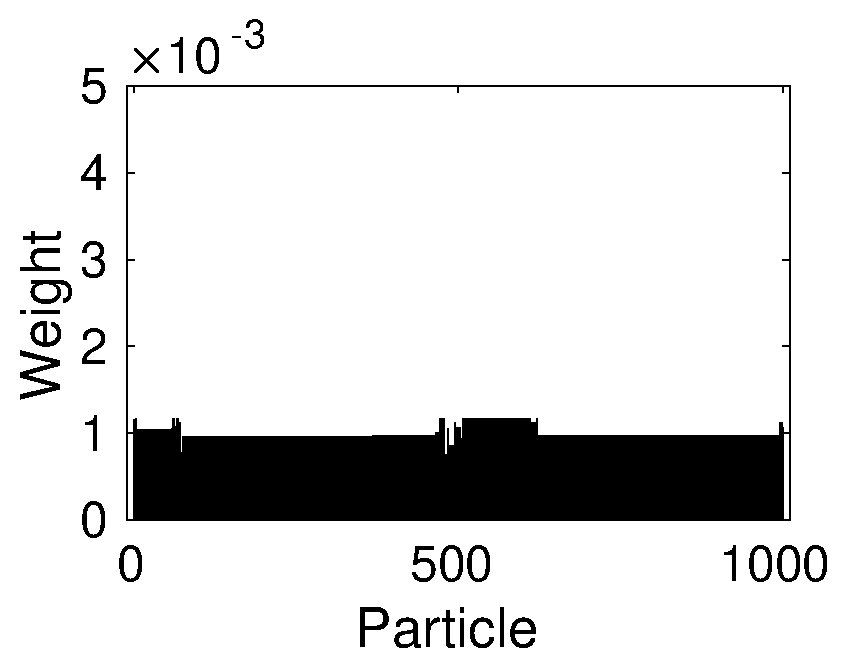
\includegraphics[scale = 0.5]{./Figures/121.eps}
		\caption*{Iterations = 121 ESS = 993.3567} 
	\end{minipage}
	\begin{minipage}{0.5\textwidth}
		\centering
		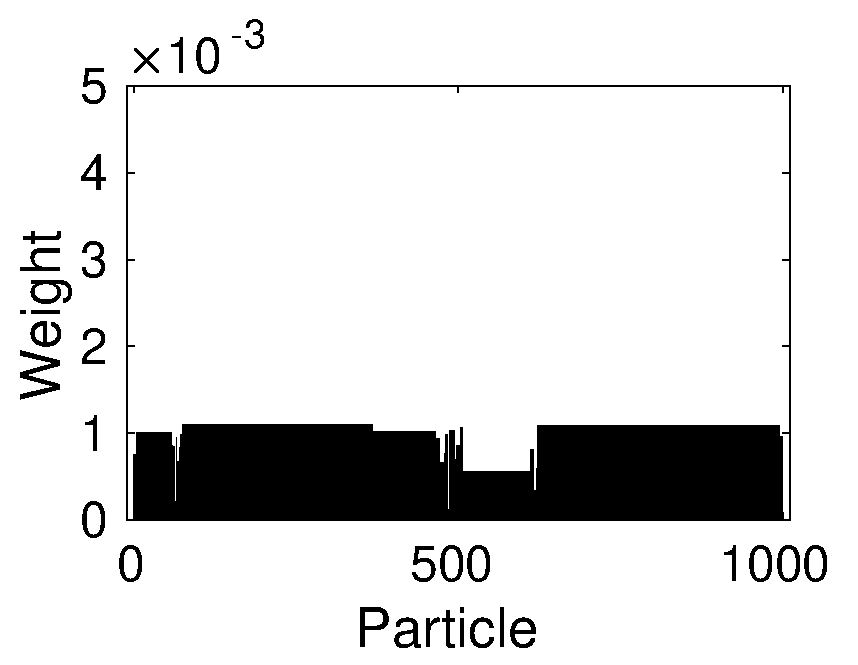
\includegraphics[scale = 0.5]{./Figures/122.eps}
		\caption*{Iterations = 122 ESS = 963.4150}
	\end{minipage}%
	\begin{minipage}{0.5\textwidth}
		\centering
		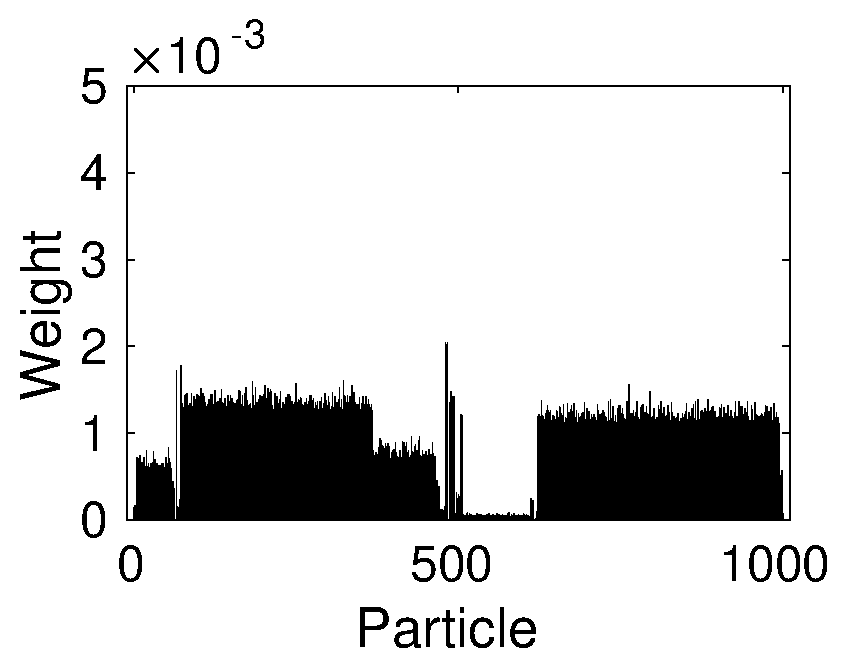
\includegraphics[scale = 0.5]{./Figures/123.eps}
		\caption*{Iterations = 123 ESS = 827.667}
	\end{minipage}
	\begin{minipage}{0.5\textwidth}
		\centering
		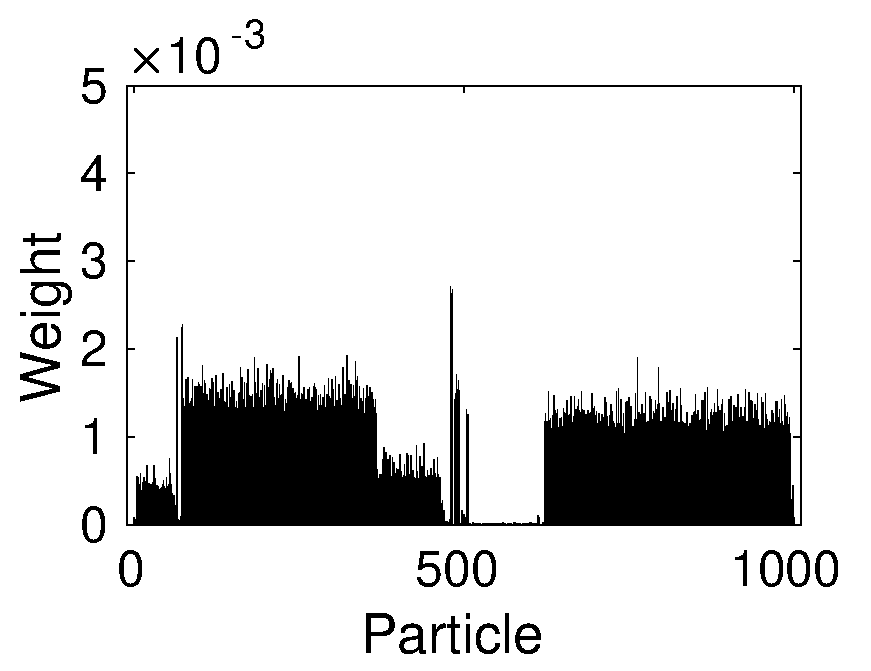
\includegraphics[scale = 0.5]{./Figures/124.eps}
		\caption*{Iterations = 124 ESS = 772.4266}
	\end{minipage}%
	\begin{minipage}{0.5\textwidth}
		\centering
		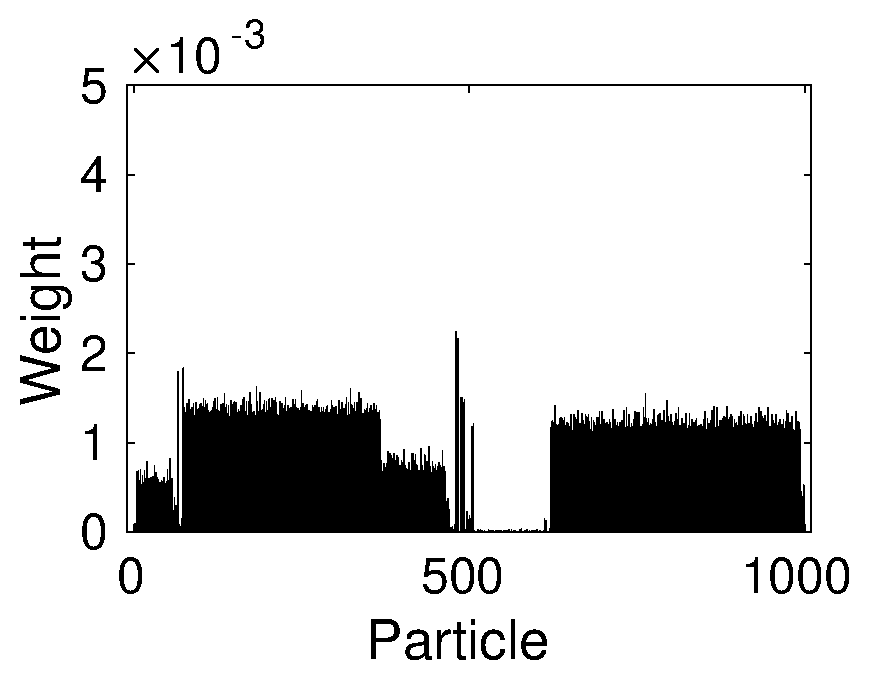
\includegraphics[scale = 0.5]{./Figures/125.eps}
		\caption*{Iterations = 125 ESS = 808.7435}
	\end{minipage}
	\caption{Normalized Weight Distribution through one re-sampling cycle(Part 1)}
	\label{fig:DGweights1}
\end{figure}
\newpage
\begin{figure}[!t]
\centering
	\begin{minipage}{0.5\textwidth}
		\centering
		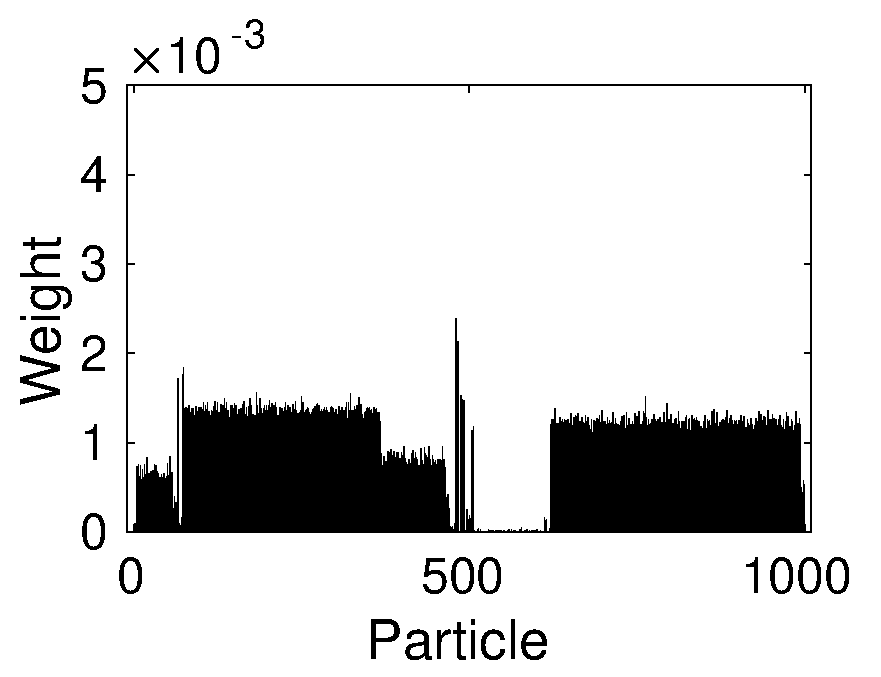
\includegraphics[scale = 0.4]{./Figures/126.eps}
		\caption*{Iterations = 126 ESS = 816.2481}
	\end{minipage}%
	\begin{minipage}{0.5\textwidth}
		\centering
		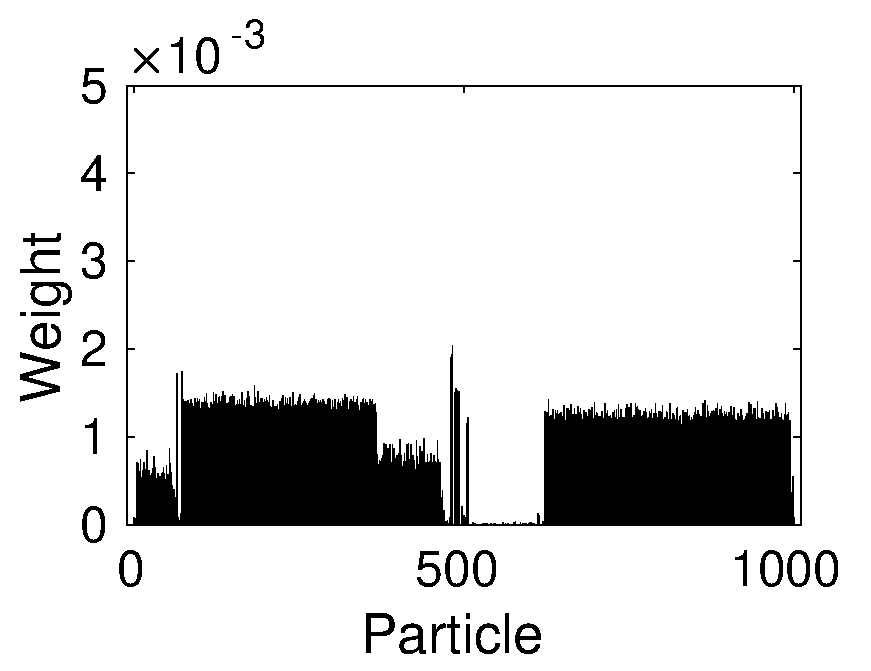
\includegraphics[scale = 0.4]{./Figures/127.eps}
		\caption*{Iterations = 127 ESS = 805.7169}
	\end{minipage}
	\begin{minipage}{0.5\textwidth}
		\centering
		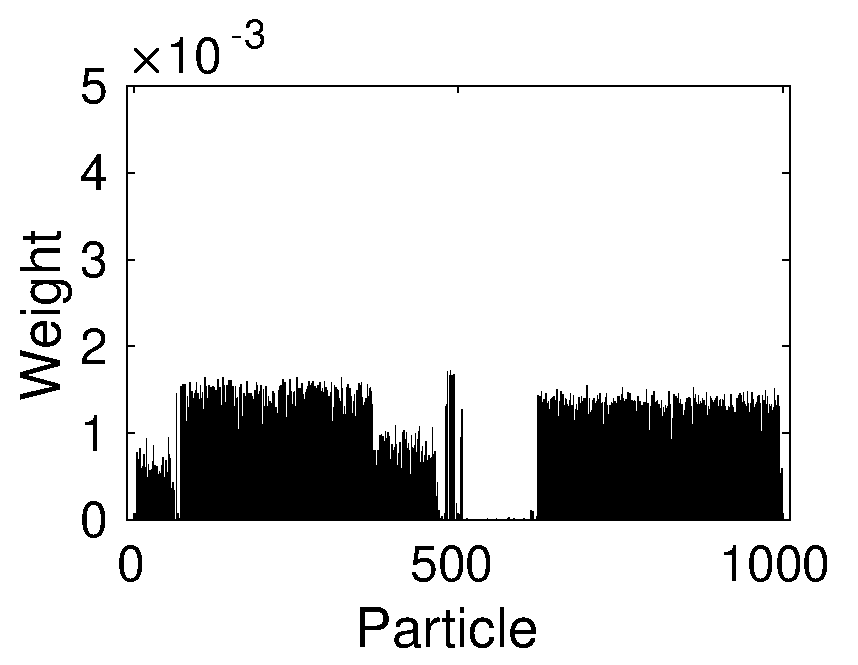
\includegraphics[scale = 0.4]{./Figures/128.eps}
		\caption*{Iterations = 128 ESS = 788.1496}
	\end{minipage}%
	\begin{minipage}{0.5\textwidth}
		\centering
		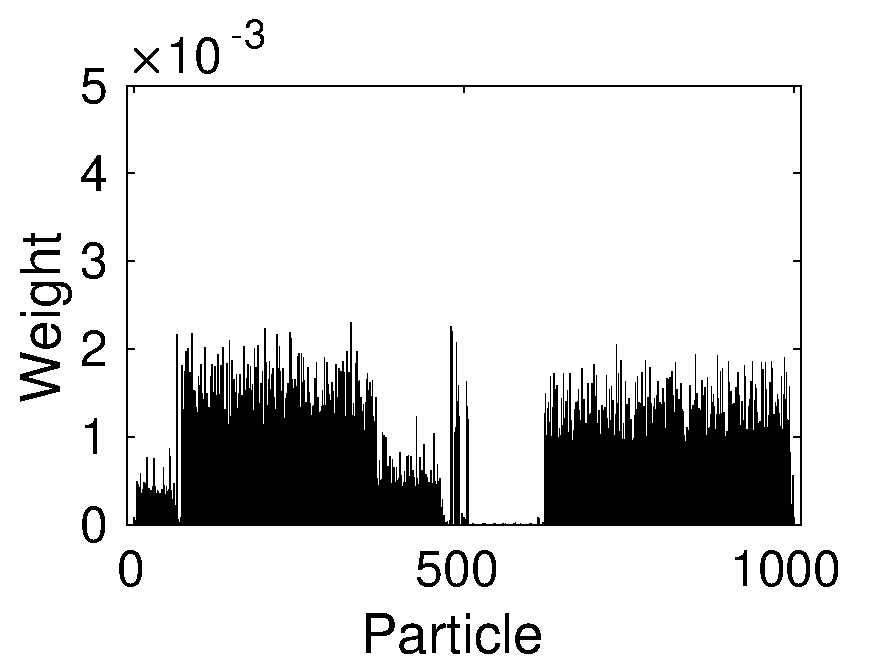
\includegraphics[scale = 0.4]{./Figures/129.eps}
		\caption*{Iterations = 129 ESS = 743.2891}
	\end{minipage}
	\begin{minipage}{0.5\textwidth}
		\centering
		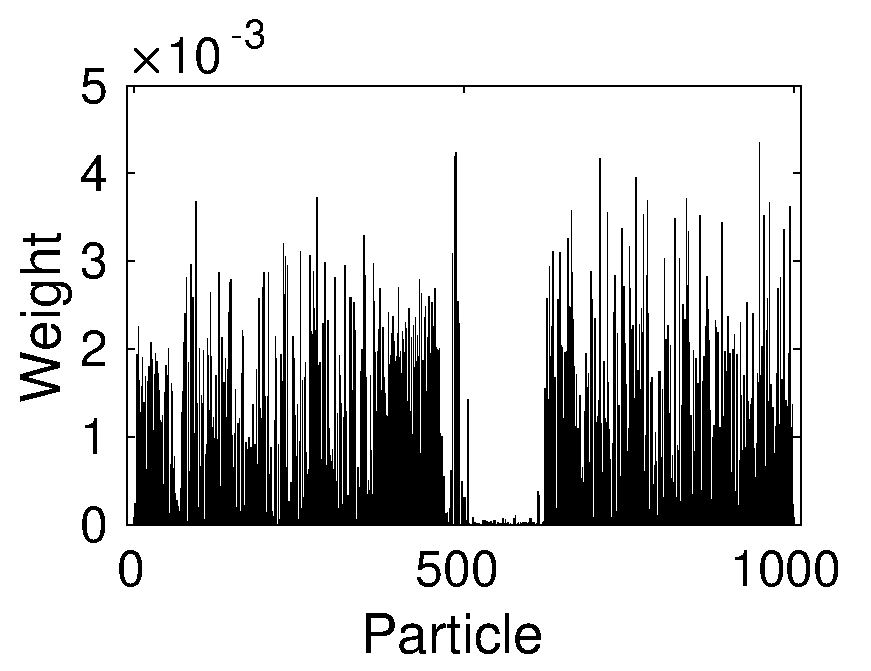
\includegraphics[scale = 0.4]{./Figures/131.eps}
		\caption*{Iterations = 131 ESS = 517.3971}
	\end{minipage}%
	\begin{minipage}{0.5\textwidth}
		\centering
		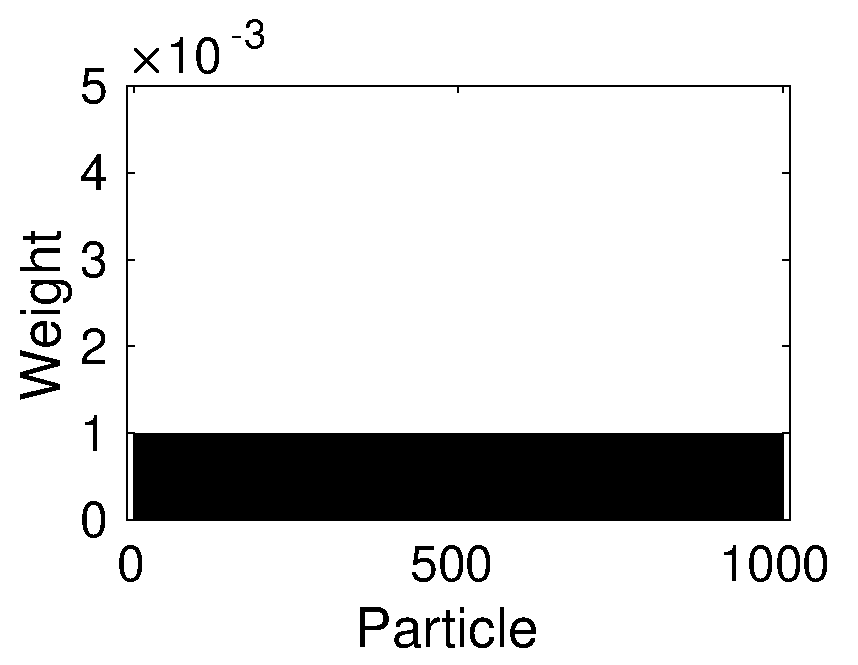
\includegraphics[scale = 0.4]{./Figures/132resampled.eps}
		\caption*{Iterations = 132 ESS = 431.4715}
	\end{minipage}
	\caption{Normalized Weight Distribution through one re-sampling cycle(Part 2)}
	\label{fig:DGweights2}
\end{figure}

\section{Conclusion}



In this report, the particle filter was used to track an object hovering over two magnets along a string. The given dataset consisted of the magnetic field strength readings experienced by the object. The implemented filter can have an in-phase and an out-of-phase tracking as shown in Figure \ref{fig:inphase} and Figure \ref{fig:outphase} due to the symmetry of the measurement data of two magnets with respect to the object being tracked.\\

The advantage of using particle filter over EKF and KF is that Particle Filter can work with state transition equations of any form and non-Gaussian noises. Recursive Bayesian estimation was used to set up a recursive relationship where the next estimate is based on the previous estimate and current measurement. Monte Carlo approximation along with importance sampling was used to weigh the samples, which are guesses of the actual state of the object. The idea of this algorithm is that the particles move to a distribution of possible new states at each time step. It is impossible to know where the system has actually transitioned to, but the hope is that some of the particles have transitioned in similar direction. An observation is taken and weights of the particles are updated based on how well its transition matches against the observation. Finally the weights are normalized so that their sum equal to 1, so that they properly represent a probability distribution. \\

This is the basic operation of the particle filter. However there is an issue. There might be certain cases where some particles move so far away that their weight approaches zero. This reduces the number of particles that contribute to the approximation of the distribution. The solution to this issue is re-sampling. Re-sampling is performed to replace particles with bad weights with particles that have good weights so that they can contribute more towards the estimation.  \\

In conclusion, particle filter is not one specific set of equation. It has many parameters other than the usual selection of model variables and equations. These include proposal distribution q() that determines the weight update equation, number of particles M, when to re-sample and re-sampling method. \\
\\
In the experiment conducted, recursive Bayesian distribution was used along with 1000 particles(M), re-sampling at 50\% ESS and select with replacement re-sampling method. \\
\\


\section*{References}
[1] \url{https://en.wikipedia.org/wiki/Particle_filter} \\
\\ \noindent
[2] \url{https://en.wikipedia.org/wiki/Importance_sampling} \\
\\ \noindent
[3] \url{http://cecas.clemson.edu/~ahoover/ece854/}
\section*{Appendix}

\subsection*{MATLAB Code}
\lstinputlisting{../asg6.m}
%--------------------------------------------------------------------------------------------------------

\end{document}
